\documentclass[12pt]{ctexart}
\usepackage{paracol}
\usepackage[most]{tcolorbox}
\usepackage{tikz}
\usetikzlibrary{hobby}
\usepackage{enumitem}
\usepackage{subcaption}
\usepackage{footnote}
\usepackage{tabularx}
\usepackage{multirow, makecell}
\usepackage{multicol}
\usepackage{caption}
\usepackage{environ}
\usepackage{booktabs}
\usepackage{geometry}
\usepackage{siunitx}
\usepackage{datatool}
\usepackage{gbt7714}
\usepackage{natbib}
\usepackage{bibentry}
\usepackage{tocbibind}
\usepackage[toc, page]{appendix}
\usepackage{xparse}
\usepackage[hidelinks]{hyperref}
\makesavenoteenv{tabular}
\makesavenoteenv{table}
\globalcounter{figure}
\bibliographystyle{gbt7714-numerical}

\hypersetup{
  bookmarksopen,
  CJKbookmarks,
  linktocpage,
  colorlinks,
  linkcolor=teal,
}

\geometry{
  left=2cm,
  right=2cm,
  top=2cm,
  bottom=2cm,
}
\setlist[itemize]{
  % align=left,
  topsep=5pt,
  itemsep=\parskip,
  font=\bfseries,
}


\renewcommand\figureautorefname{图}
\renewcommand\appendixautorefname{附录}
\renewcommand\appendixtocname{附录}
\renewcommand\appendixpagename{附录}
\settocbibname{参考文献}
\newtcolorbox{intro}[1][]{#1}
% \newcommand\bsctype[2][4]
\NewDocumentCommand { \bsctype } { D(){4} +O{} m }
  {
    \noindent
    \tcbox[
      colframe=teal, colback=teal!10,on line,
      arc=0pt, outer arc=0pt,
      boxsep=0pt, top=2pt, bottom=2pt, left=1pt, right=1pt,
      boxrule=0pt, toprule=1pt, bottomrule=1pt,
      fontupper=\itshape, width=\dimexpr#1\ccwd+2pt,
      tcbox width=forced center, #2
      ]
      {#3}
    \hspace{5pt}\ignorespaces
  }

\makeatletter
\newif\ifxtick@rotate
\tikzset{
  img/.cd,
  x/.store in=\img@x,
  y/.store in=\img@y,
  node/.store in=\img@node,
}
\tikzdeclarecoordinatesystem{img}
{%
  \tikzset{img/.cd,#1}%
  \tikz@scan@one@point\pgf@process(\img@node.south west)
  \pgf@xa=\pgf@x
  \pgf@ya=\pgf@y
  \tikz@scan@one@point\pgf@process(\img@node.north east)
  \pgfmathparse{(1-(\img@x))*\pgf@xa+(\img@x)*\pgf@x}
  \pgf@x=\pgfmathresult pt
  \pgfmathparse{(1-(\img@y))*\pgf@ya+(\img@y)*\pgf@y}
  \pgf@y=\pgfmathresult pt
}%
\NewDocumentCommand {\picgrid} {O{10} O{10} D(){} O{}} {
  \pgfkeys{/pgf/number format/.cd,fixed,fixed zerofill,precision=2}
  \foreach \i [evaluate=\i as \x using \i/#1] in {0,...,#1}
  \draw[#4]
    (img cs:node=#3, x=\x, y=0)
    node[rotate=-90, anchor=west] {\pgfmathprintnumber{\x}}
    -- (img cs:node=#3, x=\x, y=1);
  \foreach \i [evaluate=\i as \y using \i/#2] in {0,...,#2}
  \draw[#4]
    (img cs:node=#3, y=\y, x=0)
    node[left] {\pgfmathprintnumber{\y}}
    -- (img cs:node=#3, y=\y, x=1);
}

\newlength\widest
\NewEnviron{ldescription}{%
  \vbox{%
    \global\setlength\widest{0pt}%
    \def\item[##1]{%
      \settowidth\@tempdima{\textbf{##1}}%
      \ifdim\@tempdima>\widest\global\setlength\widest{\@tempdima}\fi%
    }%
    \setbox0=\hbox{\BODY}%
  }
  \begin{description}[
    leftmargin=\dimexpr\widest+0.5em\relax,
    labelindent=0pt,
    labelwidth=\widest,
    before=\begin{multicols}{2},
    after=\end{multicols}
    ]
  \BODY
  \end{description}%
}
\makeatother

\newcommand{\sortitem}[2]{%
  \DTLnewrow{list}% Create a new entry
  \DTLnewdbentry{list}{label}{#1}
  \DTLnewdbentry{list}{description}{#2}
}
\newenvironment{sortedlist}{%
  \DTLifdbexists{list}{\DTLcleardb{list}}{\DTLnewdb{list}}% Create new/discard old list
}{%
  \DTLsort*{label}{list}% Sort list
  \begingroup
  % \small
  % \begin{ldescription}
  \begin{description}[
    labelindent=0pt,
    labelwidth=.5\linewidth,
    nosep,
    font=\sffamily\bfseries,
    ]
    \DTLforeach*{list}{\mylabel=label, \mydesc=description}{%
    \item[\mylabel] \mydesc}% Print each item
  \end{description}%
  \endgroup
}

\title{轮滑手册暂行版\footnote{\url{https://github.com/ZhiyuanLck/BSC-skating-manual}}}
\author{西安交通大学轮滑社-纸鸢}
% \date{}

\begin{document}
\thispagestyle{empty}
\maketitle
\clearpage
\tableofcontents
\clearpage
\section{轮滑鞋}
\subsection{总览}
轮滑鞋分为上鞋和下鞋,以刀架为分界线,刀架以上为上鞋,包括主要的鞋体和相关的零
部件;刀架以下(包括刀架)为下鞋,主要包括刀架、轮子和把它们与上鞋相互之间连接
到一起的零部件。一般来说,不管是上鞋还是下鞋,它们的零部件都是可以更换的,包括
刀架和轮子也是可以更换的。

\bsctype(6){非一体式上鞋} 由外壳和内靴组成,大多数新手鞋都是非一体式的。

\bsctype(6){一体式上鞋} 整个上鞋是一个整体,更加能包裹双脚,使得脚对鞋的控制程
度更高。

\begin{figure}[htpb]
  \centering
  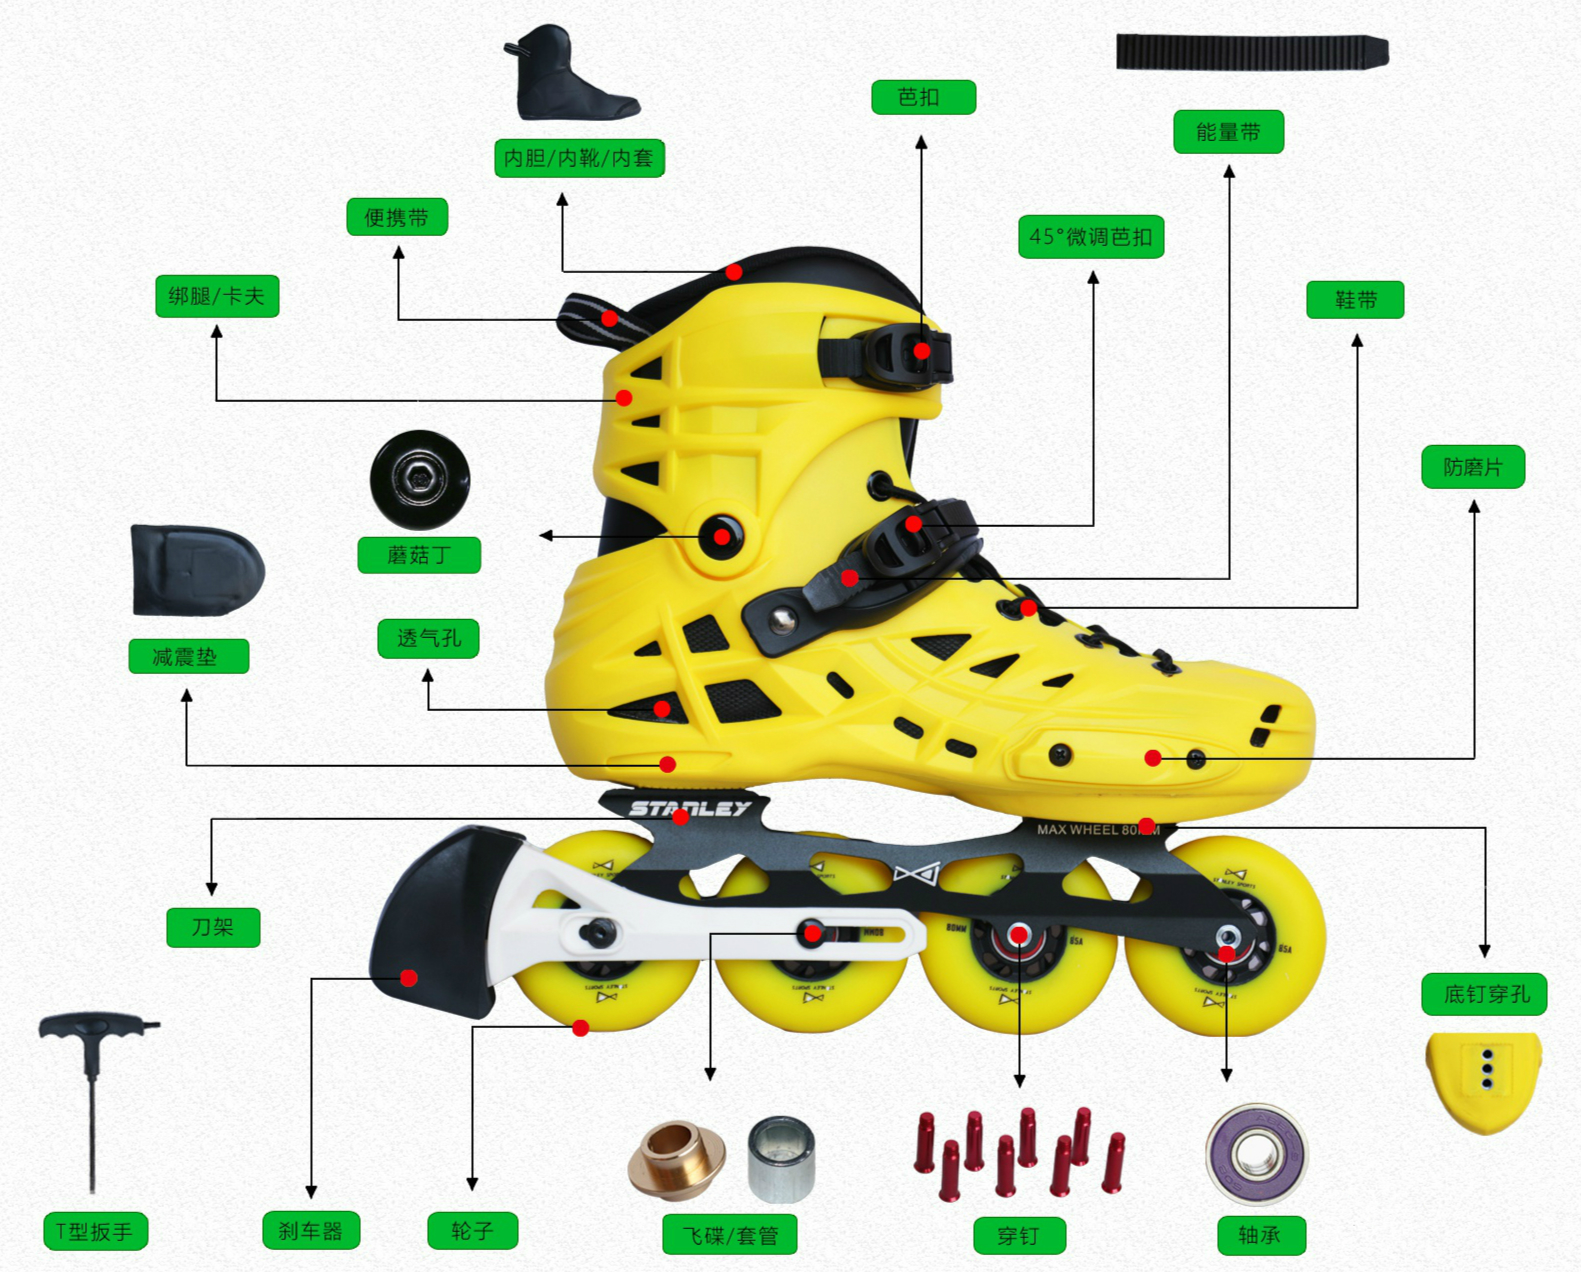
\includegraphics[width=\textwidth]{all.jpg}
  \caption{轮滑鞋组成示意图\cite{zhihu:skating1}。根据鞋的种类不同,组成部分略
  有不同,比如花式轮滑、速滑使用的轮滑鞋\textcolor{red}{没有刹车器},进阶鞋的
上鞋大多数不是硬壳,有些鞋也并没有防磨片等等。}
\end{figure}
\clearpage
\begin{paracol}{2}
\switchcolumn[0]*
\switchcolumn[0]*[\subsection{刀架}]
\begin{intro}
  常见类型:平架、香蕉架
  \begin{itemize}[labelindent=1em, itemindent=!]
    \item[平架] 四个穿孔在同一高度
    \item[香蕉架] 中间二孔低于前后二孔
  \end{itemize}
  常见尺寸:231\si{mm}、243\si{mm}

  231\si{mm}刀架最大可装$4\times 76$\si{mm}轮

  243\si{mm}刀架最大可装$4\times 80$\si{mm}轮

  刀架与上鞋通过底钉连接
\end{intro}
\autoref{fig:daojia}~上图为刀架实体,下图为平架和香蕉架示意图,一般来说,香蕉架
前后两孔比中间两孔高\si{4mm}。

\begin{rightcolumn}
\begin{figure}[htpb]
\centering
\begin{tikzpicture}[scale=.4]
\node[inner sep=0pt, anchor=south] at (9, 8)
  {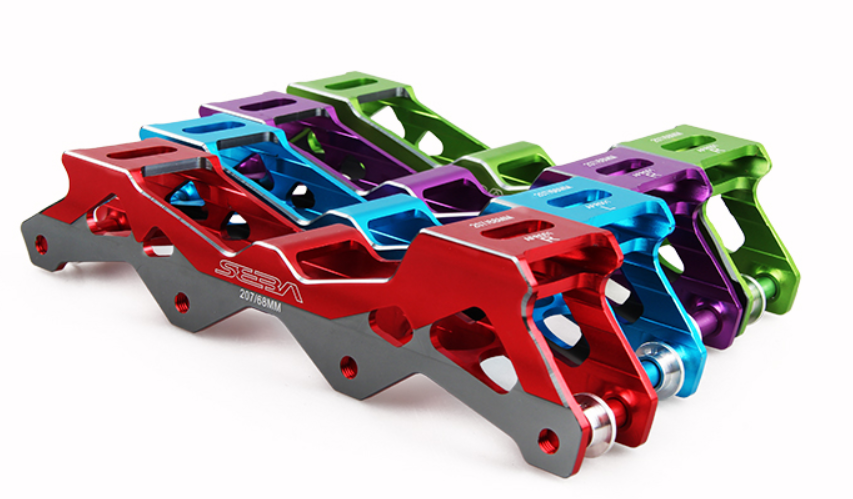
\includegraphics[width=0.8\linewidth]{daojia.png}};
\fill[teal]
  (0, 0) -- (1, 4) -- ++(3, 0) arc (-110:-40:8) -- ++(3, 0) -- (18, 0) --
  ++(-1.5, 0) coordinate (a1) -- ++(120:2) -- ++(-1.5, 0) -- ++(-120:2) --
  ++(-1.5, 0) coordinate (a2) -- ++(120:2) -- ++(-1.5, 0) -- ++(-120:2) --
  ++(-1.5, 0) coordinate (a3) -- ++(120:2) -- ++(-1.5, 0) -- (2, 0) --cycle
  ;
\path ([shift={(0.5, 1)}]a1) coordinate (b1);
\path ([shift={(0.75, 1)}]a2) coordinate (b2);
\path ([shift={(0.75, 1)}]a3) coordinate (b3);
\path (1.4, 1) coordinate (b4);
\path (b4) ++(70:1) coordinate (c4);
\path (b1) ++(110:1) coordinate (c1);
\draw[red, very thick] (b1) -- (b2) -- (b3) -- (b4);
\draw[green, very thick] (c1) -- (b2)(b3) -- (c4);
\fill[black] (b1) circle (3mm);
\fill[black] (b2) circle (3mm);
\fill[black] (b3) circle (3mm);
\fill[black] (b4) circle (3mm);
\fill[yellow] (c4) circle (3mm);
\fill[yellow] (c1) circle (3mm);
\end{tikzpicture}
\caption{刀架}
\label{fig:daojia}
\end{figure}
\end{rightcolumn}
\switchcolumn[0]*[\subsection{轮子}]
轮子通过穿钉固定在刀架上。轮子内部较硬的部分是安装轴承的,被称为“内扣”也叫“轮
毂”,轮子外侧是接触地面的部分,被称为“轮肉”。

一只轮滑鞋上的轮子一般为$3\sim 5$个不等。根据轮子的大小、软硬成都、材质或者是
否可以闪光可以把它们分为不同的种类。
\begin{rightcolumn}
\begin{figure}[htpb]
  \centering
  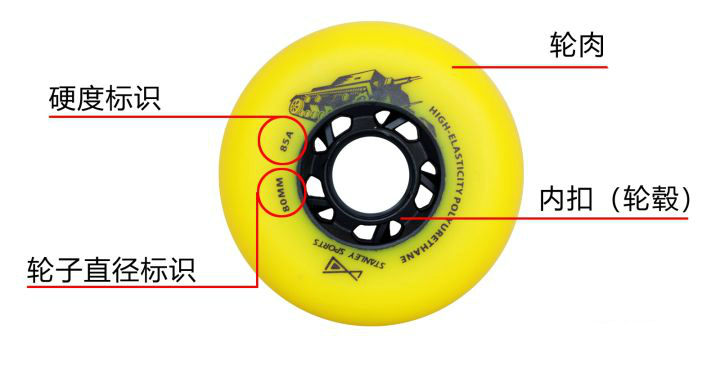
\includegraphics[width=\linewidth]{lunzi.jpg}
  \caption{轮子示意图\cite{zhihu:skating1}}
\end{figure}
\end{rightcolumn}
\end{paracol}
\bsctype{轮子大小}不同大小的轮子适应不同的场合,\autoref{fig:lunzi_type}~给出了详细的说明,对于自
由式轮滑\footnote{自由式轮滑,或称滚轴平地花式,是现代轮滑竞技项目之一,由四大
项目 – 花式绕桩、速度过桩、花式刹停、自由跳高所组成。}来说,轮子直径一般为
64-80\si{mm},64-70\si{mm}一般用在儿童鞋上,72-80\si{mm}一般用在成人鞋上。

\begin{figure}[htpb]
  \centering
  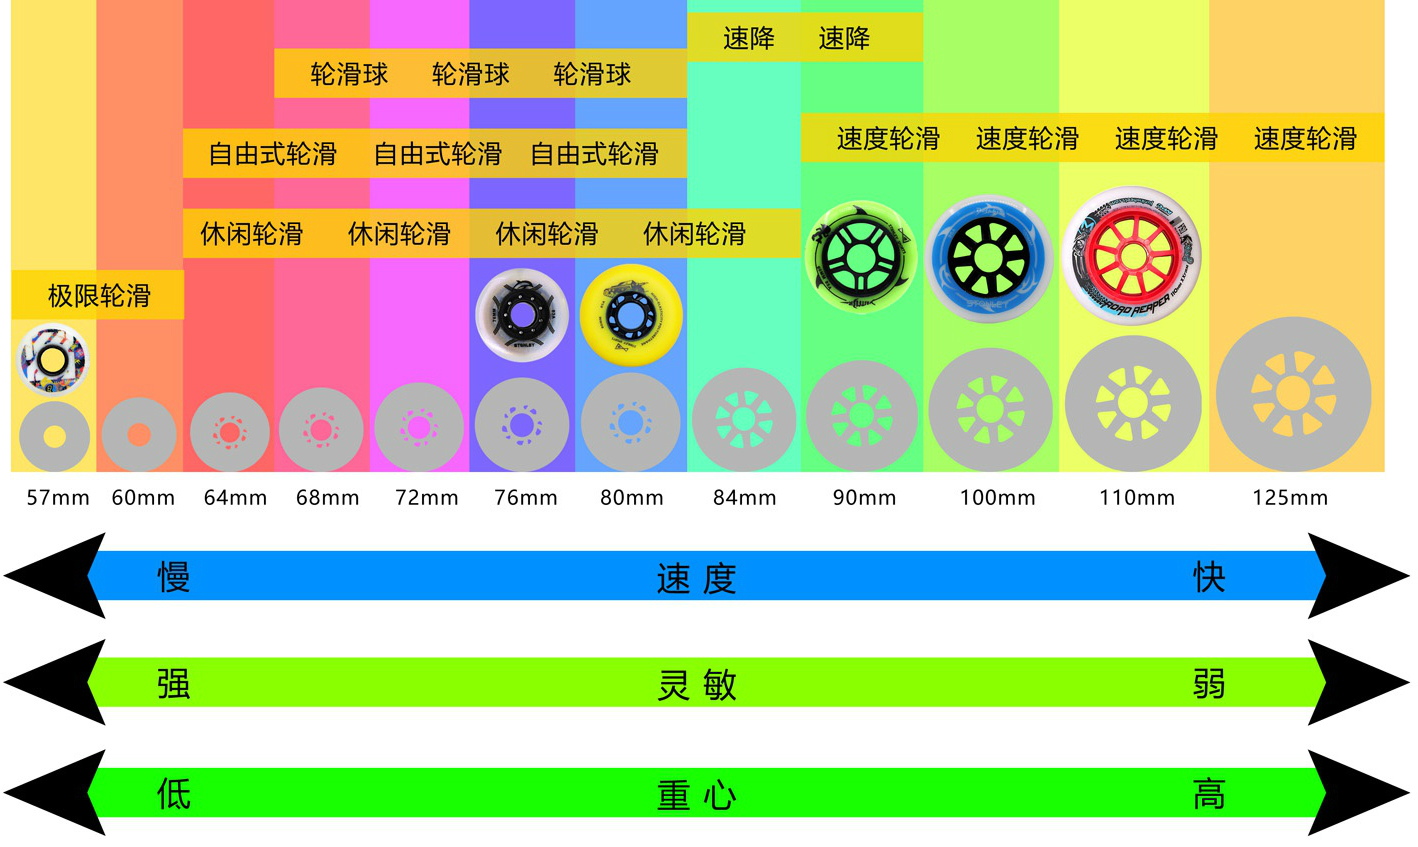
\includegraphics[width=\linewidth]{lunzi_type.jpg}
  \caption{轮滑鞋轮子的尺寸、使用范围和特点\cite{zhihu:skating1}}
  \label{fig:lunzi_type}
\end{figure}

\bsctype{轮子软硬}轮子上的轮肉使用不同的材质,它的软硬、弹性不同。在轮子上通常表示为一个数字+A
(比如76A、80A、85A)。轮子越软,抓地性能越好,应根据自身需要和使用场景选择合
适软硬程度的轮子。比如说花式刹停,刹车的距离是比赛非常重要的因素,这就需要轮子
接触地面时不能抓地,而要有“漂”的感觉,所以刹车时用的轮子一般的偏硬而且不抓地。

\bsctype{轮子软硬}轮子轮肉的材质目前最普遍的是PU、TPU、PVC。PVC轮子俗称塑料轮,主要是几十元、一
两百元的轮滑鞋上使用较多。这种PVC轮子材质过硬,几乎不抓地,容易打滑、也没有弹
性和减震作用。可能唯一的优点就是价格便宜了。TPU、PU轮俗称为橡胶轮。PU是聚氨酯,
TPU是热塑性聚氨酯,都是一种复合材质。TPU和PU本质上是同一种材料所组成的。但是所
用的配方不是一样的所以性能也有区别。使用不同配方的材质会导致轮子的抓地、弹性、
摩擦力不同。\textcolor{red}{推荐选购PU、TPU材质的轮子。}

\bsctype{闪光轮}闪光轮的本质是在轮子装了线圈,然后将轮子里的轴承作为带有磁性的磁芯,磁场切割线
圈会产生能量,这个能力就让轮子内的灯发光了。闪光轮虽然好看,但是会%
\textcolor{red}{滑起来更费劲一些}。

\subsection{轴承}
\subsubsection{轴承架构}
\bsctype{防尘盖}防尘盖是轮滑轴承盖住内部滚珠的圆形盖子,作用是防止轴承内部进入
异物。
\begin{figure}[tb]
\centering
\begin{tikzpicture}[font=\large, img/node=a]
  \node[inner sep=0pt] (a) {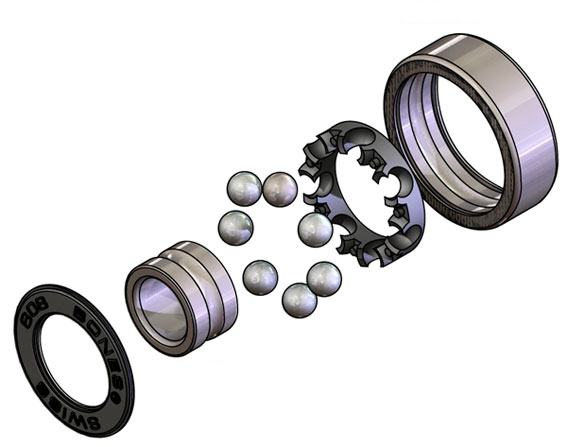
\includegraphics[width=0.8\linewidth]{bearing.jpg}};
  % \picgrid[20][20](a)[red]
  \node at (img cs:x=0.1, y=0.45) {防尘盖};
  \node at (img cs:x=0.35, y=0.15) {内圈};
  \node at (img cs:x=0.46, y=0.7) {滚珠};
  \node at (img cs:x=0.68, y=0.34) {保持架};
  \node at (img cs:x=0.8, y=1) {外圈};
\end{tikzpicture}
\caption{轴承架构\cite{zhihu:migao}}
\end{figure}

\bsctype{轴承外圈}作为轴承与轮滑鞋轮子直接接触的部分,主要是起支撑作用,承受来
自轮子的直接压力。

\bsctype{滚珠}起滚动和传递力的作用。滚珠的大小、数量、质量,决定着轮滑轴承的载
荷力和运转的性能。

\bsctype{保持架}隔离和固定各滚珠位置,起到减少滚珠之间的摩擦力,尽可能的让每个
滚珠之间载荷相同和引导滚珠正常运行的作用。

\bsctype{轴承内圈}轮滑轴承与刀架穿钉接触的部分,与外圈一同构成滚珠的轨道。

\subsubsection{轴承分类}
\begin{figure}[tb]
  \centering
  \subcaptionbox{碳钢轴承}{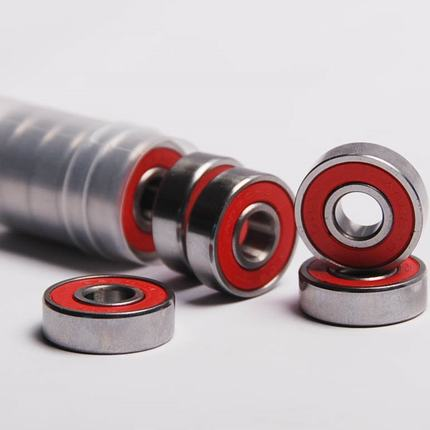
\includegraphics[width=.3\linewidth]{tangang.jpg}}
  \subcaptionbox{铬钢轴承}{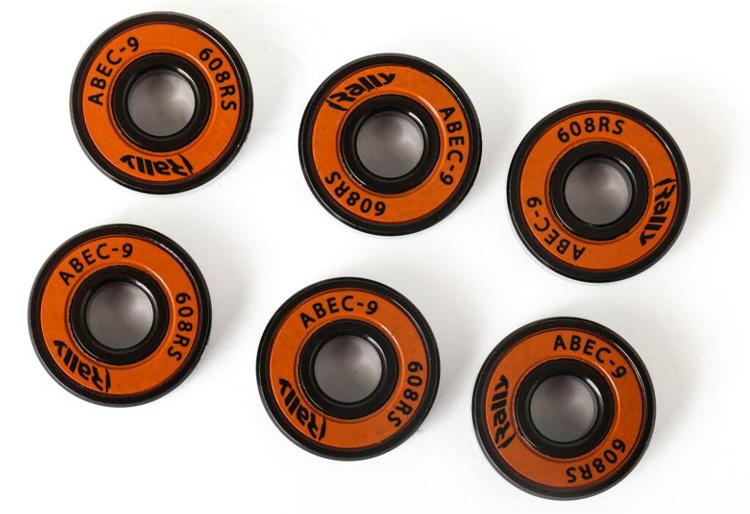
\includegraphics[width=.3\linewidth]{gegang.jpg}}
  \\
  \subcaptionbox{钛合金轴承}{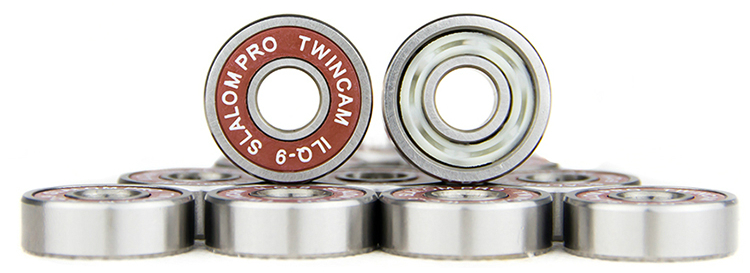
\includegraphics[width=.3\linewidth]{ti.jpg}}
  \subcaptionbox{陶瓷轴承}{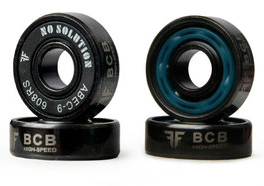
\includegraphics[width=.3\linewidth]{heitao.jpg}}
  \caption{不同种类的轴承\cite{zhihu:migao}}
\end{figure}

\bsctype(5){碳钢轴承}碳钢轴承成本低廉,但硬度低,耐磨性较差,使用寿命在常见轮
滑轴承里面也是最短的。

\bsctype(5){铬钢轴承}市场上轮滑鞋中最为常见的轴承,其硬度高,耐磨性强,抗压性
能优秀。适用于平常喜欢平花刹停的玩家。

\bsctype(5){钛合金轴承}用于高端FSK(自由轮滑)的顶级轴承,强度高,抗压耐磨性极
佳。适合热衷于各种剧烈FSK动作和花式刹停的玩家。

\bsctype(5){陶瓷轴承}分为黑陶轴承和白陶轴承,这两者滚珠摩擦力极小,都具有转速
高、硬度强、耐高温、耐腐蚀性强、无油自润滑等优点,唯一的区别是白陶轴承硬度略低
于黑陶,适合喜好速滑的玩家,但是不适合平花刹停的玩家。

\subsubsection{轮滑轴承尺寸}

\bsctype(3){608}用于美国制造的双排轮滑鞋和所有单排轮滑鞋以及所有滑板和长板。

\bsctype(3){627}用于意大利制造的高端的花样轮滑鞋和双排速度轮滑鞋。

\bsctype(3){688}用于一些新型的速滑轮。

\bsctype(3){698}用于一些新型的速滑轮。

\begin{paracol}{2}
\begin{leftcolumn}
\begin{table}[htb]
  \caption{轴承规格\cite{quad, liveaboutdotcom}}
  \centering
  \begin{tabular}{>{\bfseries}ccccc}
    \toprule
    代号 & 内径 & 外径 & 高度\footnote{无防尘} & 高度{*}\footnote{双面防尘}\\
    \midrule
    608 & 8mm & 22mm & 7mm & 7mm\\
    627 & 7mm & 22mm & 7mm & 7mm\\
    688 & 8mm & 16mm & 4mm & 5mm\\
    698 & 8mm & 19mm & 6mm & 6mm\\
    \bottomrule
  \end{tabular}
\end{table}
\end{leftcolumn}
\begin{rightcolumn}
\centering
\vspace{\intextsep}
\captionsetup{type=figure}
\begin{tikzpicture}[img/node=a]
  \node[inner sep=0pt] (a) {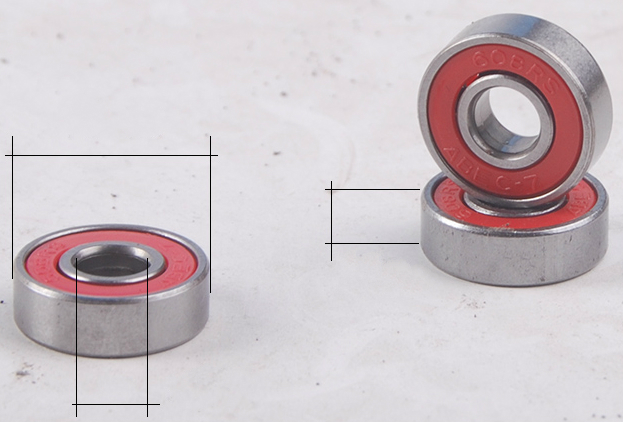
\includegraphics[width=\linewidth]{size.jpg}};
  % \picgrid[20][20](a)[red, font=\scriptsize]
  \node[anchor=west] at (img cs:x=0.3, y=0.05) {内径8\si{mm}};
  \node at (img cs:x=0.18, y=0.7) {外径22\si{mm}};
  \node[align=center] at (img cs:x=0.45, y=0.5) {高度\\7\si{mm}};
\end{tikzpicture}
\caption{608轴承}
\label{fig:size}
\end{rightcolumn}
\switchcolumn*[
代号后面可能会有后缀字母,Z代表单面防尘,ZZ代表双面防尘,2RS/RS/RZ代表有密封
圈,BRS代表有密封圈且防水。对于自由式轮滑来说,608轴承较为常见(见
\autoref{fig:size})。
]
\end{paracol}

\subsubsection{轮滑轴承ABEC标准}
  ABEC标准\cite{wiki:abec}是为精密轴承在生产制造时使用的公差分出不同等级而设计
  一套标准。公差指滚珠球体和滑轨之间的空间,公差越小,轴承的精度和效率越高(并
  不意味这更快)。ABEC标准用奇数定义了5个类别(1,3,5,7,9),类别越高,公差
  越小。基于ABEC标准的轴承有7个滚珠。

\subsubsection{轮滑轴承ILQ标准}
  严格来说ILQ是轴承厂商TWINCAM旗下的一个品牌,它的分级和ABEC类似,不同的是ILQ
  系列的轴承只有6个滚珠

\subsection{其他零部件}
\begin{paracol}{2}
  \bsctype{飞碟/套管}飞碟/套管安装在轮子内,介于轮子上两个轴承中间的位置,主要
  作用是让轮子能够更好的旋转。

  \bsctype{穿钉}穿钉是将轮子、刹车器固定在刀架上的零件。穿钉分为单面穿钉和双面
  穿钉。通常使用塑料刀架的轮滑鞋多配双面穿钉,双面穿钉指的是一个螺丝,一个螺帽。
  螺丝穿过轮子和刀架上的孔,拧在螺帽上。单面穿钉多用在铝合金刀架上,单面穿钉穿
  过刀架的一侧和轮子直接拧在刀架另一侧孔的螺纹上。
\begin{rightcolumn}
\begin{figure}[tb]
\centering
\begin{tikzpicture}[img/node=a, font=\small]
  \node[inner sep=0pt] (a) {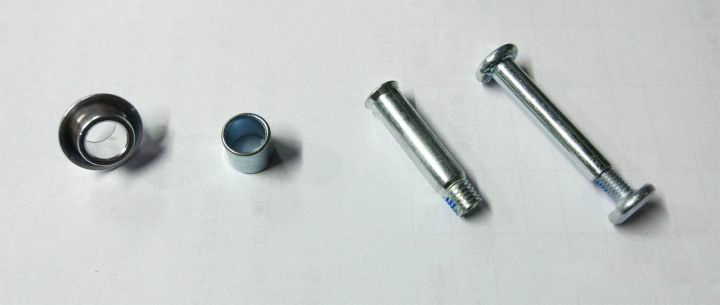
\includegraphics[width=\linewidth]{other.jpg}};
  % \picgrid[20][20](a)[red, font=\tiny]
  \node at (img cs:x=0.15, y=0.15) {飞碟};
  \node at (img cs:x=0.35, y=0.15) {套管};
  \node at (img cs:x=0.59, y=0.15) {单面穿钉};
  \node at (img cs:x=0.8, y=0.15) {双面穿钉};
\end{tikzpicture}
\caption{其他零部件}
\end{figure}
\end{rightcolumn}
\end{paracol}

\section{花式绕桩Freestyle Slalom}
\subsection{技术特点}
花式绕桩是滚轴溜冰的Flat Land,主要集中地面上的技巧,现时花式绕桩的技术被分成
了5种\cite{wiki:skating}:

\bsctype(2){其他}泛指任何四大类以外的绕桩动作

\bsctype(2){蹲坐}蹲坐指绕桩时膝盖折幅达到臀部比膝盖低的动作

\bsctype(2){跳跃}跳跃指绕桩时会有双脚同时离地的动作

\bsctype(2){直线}直线系前称“单轮系”,现时将所有踪向过桩的动作整合为直线类,其
中单轮指以一个轮子完成的动作,为花式绕桩中难度系数最高的技术,几乎所有最难的招
式都是以单轮的方式作出,亦是花式绕桩中最广为人知、最有“平花味”的动作。

\bsctype(2){旋转}旋转指持续以画圆周或自体为圆心方式旋转的动作

\subsection{动作技术等级}
目前花式绕桩动作被分为5个等级(A-E),A等级最难,E等级最简单,每个等级又被分为
十个小级\footnote{WSSA \emph{Inline Freestyle RuleBook 2020}: \url{https:%
//www.worldslalomseries.com/app/download/11425432095/INLINE+FREESTYLE+RULEBOOK+2020+new.pdf?
t=1584628122}}(见\autoref{app:rank}),所有动作都以在80\si{cm}桩距的桩上平稳、匀速
完成4个桩或绕桩转3圈作为评分的最低标准。

\subsection{视频教学资料}
\href{https://www.youtube.com/channel/UCgE0Xdh91jMPX-A8nyxPe_w/videos}{WSSA自
由式轮滑动作分解}\footnote{\url{https://www.youtube.com/channel/UCgE0Xdh91jMPX-A8nyxPe_w/videos}}
,由国内顶尖轮滑运动员演示的演示视频,主要用作演示。

\clearpage
\bibliography{skating}

\clearpage
\begin{appendices}
  \section{花式绕桩动作等级表}
  \label{app:rank}
  \noindent
\begingroup
\let\mc\multicolumn
\tiny
\begin{tabularx}{\linewidth}{Xr*{5}{c}rX}
  \toprule
  % && \mc1c{其他类} & \mc1c{蹲坐类} & \mc1c{跳跃类} & \mc1c{单轮类} & \mc1c{旋
  % 转类} &&\\
  && 其他类 & 蹲坐类 & 跳跃类 & 直线类 & 旋转类 &&\\
  \midrule
  \multirowcell{10}{A\\(50-60)}
  & 10 && 单轮天国向后 &&& 单轮茶壶转 & 10 &
  \multirowcell{10}{A\\(50-60)} \\
  & 9 && 单轮天国向前 & 单轮Wiper &&& 9 & \\
  & 8 &&&&&& 8 & \\
  & 7 &&&&&& 7 & \\
  & 6 &&&&&& 6 & \\
  & 5 &&&&& 单轮后内刃/后外刃单桩转& 5 & \\
  & 4 & 天鹅蟹 & 单轮茶壶向后 &&& 单轮后内刃/后外刃过桩转 & 4 & \\
  & 3 &&&&&& 3 & \\
  & 2 &&&& 单轮Special/单轮摆摆系列 & 单轮前内刃/外刃过桩转 & 2 & \\
  & 1 && 超人单轮茶壶 &&&& 1 & \\
  \midrule
  \multirowcell{10}{B\\(40-50)}
  & 10 && 单轮茶壶向前 && 单轮连续转向系列 & 单轮前内刃/外刃单桩转 & 10 &
  \multirowcell{10}{B\\(40-50)} \\
  & 9 &&& 茶壶连续转向跳 &&& 9 & \\
  & 8 &&& 茶壶跳向后 &&& 8 & \\
  & 7 & 双轮内蟹 & 天国向后 &&&& 7 & \\
  & 6 &&&&&& 6 & \\
  & 5 &&&&&& 5 & \\
  & 4 &&&&&& 4 & \\
  & 3 &&&&&& 3 & \\
  & 2 & 交叉玛丽向后 &&&&& 2 & \\
  & 1 &&&& 单轮捅捅 && 1 & \\
  \midrule
  \multirowcell{10}{C\\(30-40)}
  & 10 && 天国向前 && 单轮向后 && 10 &
  \multirowcell{10}{C\\(30-40)} \\
  & 9 & 交叉玛丽向前 & 茶壶向后 & 茶壶跳向前 && 黑天鹅过桩转 & 8 & \\
  & 8 & 内蟹 &&&& 天鹅单桩转 & 7 & \\
  & 7 &&&&& 天鹅过桩转 & 6 & \\
  & 6 & 双轮蟹 &&& 单脚连续正/反转向 && 5 & \\
  & 5 &&&& 单轮向前 & 双轮转 & 5 & \\
  & 4 &&& Wiper &&& 4 & \\
  & 3 && 蹲坐交叉玛丽向后 &&& 反Q转 & 3 & \\
  & 2 & Z-蟹步 & 茶壶向前 &&&& 2 & \\
  & 1 && 蹲坐交叉玛丽向前 & 脚尖X跳 &&& 1 & \\
  \midrule
  \multirowcell{10}{D\\(20-30)}
  & 10 & 脚尖X && 单脚连续转向跳 &&& 10 &
  \multirowcell{10}{D\\(20-30)} \\
  & 9 & 刷子 &&&& 正Q转 & 9 & \\
  & 8 & 玛丽Special & 蹲坐玛丽向后 &&& 双脚转 & 8 & \\
  & 7 & 蟹步/蟹剪 & 蹲坐玛丽向前/Full Remi &&& 双脚连续转向 & 7 & \\
  & 6 &&&& 玛丽向后 && 6 & \\
  & 5 &&&&&& 5 & \\
  & 4 &&&& 风车系列/Sweepers && 4 & \\
  & 3 &&&&&& 3 & \\
  & 2 &&&&&& 2 & \\
  & 1 &&&&&& 1 & \\
  \midrule
  \multirowcell{10}{E\\(10-20)}
  & 10 & 画八 & 小汽车/5轮蹲坐 &&&& 10 &
  \multirowcell{10}{E\\(10-20)} \\
  & 9 & 反画八 &&& 单脚向后 & 意大利人/Volt & 9 & \\
  & 8 & 太空步 && X跳 &&& 8 & \\
  & 7 &&& 蟹交叉跳 &&& 7 & \\
  & 6 &&&&& Crazy Sun/墨西哥人& 6 & \\
  & 5 & 漫步向前/后 &&&&& 5 & \\
  & 4 & (Double) Crazy系列 &&&& 太阳花/盘藤 & 4 & \\
  & 3 & 恰恰/X && 蟹绕桩跳 & 单脚向前 && 3 & \\
  & 2 & 尼尔森向前/后 &&&&& 2 & \\
  & 1 && 蹲坐鱼形向前 && 交叉/蛇行/鱼行系列 && 1 & \\
  \midrule
  && 其他类 & 蹲坐类 & 跳跃类 & 直线类 & 旋转类 &&\\
  \bottomrule
\end{tabularx}
\endgroup

  \clearpage
  \section{花式绕桩动作术语表}
  \begin{sortedlist}
  \sortitem{Toe Christie Back}{单轮天国向后}
  \sortitem{Toe Footgun Spin}{单轮茶壶转}
  \sortitem{Toe Christie}{单轮天国向前}
  \sortitem{Toe Wiper}{单轮Wiper}
  \sortitem{Butterfly}{天鹅蟹}
  \sortitem{Toe Footgun Back}{单轮茶壶向后}
  \sortitem{Internal 1 Cone 7 Back}{单轮后内刃单桩转}
  \sortitem{External 1 Cone 7 Back}{单轮后外刃单桩转}
  \sortitem{Internal Backward 7}{单轮后内刃过桩转}
  \sortitem{External Backward 7}{单轮后外刃过桩转}
  \sortitem{Internal 7}{单轮前内刃单桩转}
  \sortitem{External 7}{单轮前外刃单桩转}
  \sortitem{Wheeling Special}{单轮Special}
  \sortitem{Wheeling Shifts}{单轮摆摆}
  \sortitem{Superman}{超人单轮茶壶}
  \sortitem{Toe Footgun}{单轮茶壶向前}
  \sortitem{Flipping 360 Shift}{单轮连续转向}
  \sortitem{Internal 1 Cone 7}{单轮前内刃单桩转}
  \sortitem{External 1 Cone 7}{单轮外内刃单桩转}
  \sortitem{Footgun Footspin}{茶壶连续转向跳}
  \sortitem{Kazatchok Back}{茶壶跳向后}
  \sortitem{Toe Reverse Eagle}{双轮内蟹}
  \sortitem{Christie Back}{天国向后}
  \sortitem{Cobra Back}{交叉玛丽向后}
  \sortitem{Sewing Machine}{单轮捅捅}
  \sortitem{Christie}{天国向前}
  \sortitem{Wheeling Back}{单轮向后}
  \sortitem{Cobra}{交叉玛丽向前}
  \sortitem{Footgun Back}{茶壶向后}
  \sortitem{Kazatchok}{茶壶跳向前}
  \sortitem{Cross Korean Volt Back}{黑天鹅过桩转}
  \sortitem{Reverse Eagle}{内蟹}
  \sortitem{One Cone Cross Korean Volt}{天鹅单桩转}
  \sortitem{Cross Korean Volt}{天鹅过桩转}
  \sortitem{Flat Shift}{单脚连续正转向}
  \sortitem{Flat Fake}{单脚连续反转向}
  \sortitem{Toe Wheeling Eagle}{双轮蟹}
  \sortitem{Wheeling Forward}{单轮向前}
  \sortitem{Two Wheels Spinning}{双轮转}
  \sortitem{Cross Sitting Heel-Toe Back}{蹲坐交叉玛丽向后}
  \sortitem{Reverse J-Turn}{反Q转}
  \sortitem{Z-Eagle}{Z-蟹步}
  \sortitem{Footgun}{茶壶向前}
  \sortitem{Cross Sitting Heel Toe}{蹲坐交叉玛丽向前}
  \sortitem{Special Jumps}{脚尖X跳}
  \sortitem{Special}{脚尖X}
  \sortitem{Footspin}{单脚连续转向跳}
  \sortitem{Brush}{刷子}
  \sortitem{J-Turn}{正Q转}
  \sortitem{Heel Toe Special}{玛丽Special}
  \sortitem{Sitting Heel-Toe Back}{蹲坐玛丽向后}
  \sortitem{2 Feet Spin}{双脚转}
  \sortitem{Eagle}{蟹步}
  \sortitem{Eagle Cross}{蟹剪}
  \sortitem{Sitting Heel-Toe}{蹲坐玛丽向前}
  \sortitem{Total Cross}{双脚连续转向}
  \sortitem{Heel-Toe Back}{玛丽向后}
  \sortitem{Fan Volt}{风车}
  \sortitem{Eight}{画八}
  \sortitem{Small Car}{小汽车}
  \sortitem{5 Wheels Sitting}{5轮蹲坐}
  \sortitem{Eight Back}{反画八}
  \sortitem{One Foot Back}{单脚向后}
  \sortitem{Italian}{意大利人}
  \sortitem{Crazy Legs}{太空步}
  \sortitem{X Jump}{X跳}
  \sortitem{Crab Cross}{蟹交叉跳}
  \sortitem{Stroll}{漫步向前}
  \sortitem{Back Stroll}{漫步向后}
  \sortitem{Mexican}{墨西哥人}
  \sortitem{Sun}{太阳花}
  \sortitem{Mabrouk}{盘藤}
  \sortitem{Chap Chap}{恰恰}
  \sortitem{Crab}{蟹绕桩跳}
  \sortitem{One Foot}{单脚向前}
  \sortitem{Nelson}{尼尔森向前}
  \sortitem{Nelson Back}{尼尔森向后}
  \sortitem{Sitting Fish}{蹲坐鱼形向前}
  \sortitem{Cross}{交叉向前}
  \sortitem{Snake}{蛇形向前}
  \sortitem{Fish}{鱼行向前}
\end{sortedlist}

\end{appendices}
\end{document}
